% Chapter 8

\chapter{Integration of DJANGOH in the Monte-Carlo Chain} % Chapter title

\label{ch:MC} % For referencing the chapter elsewhere, use \autoref{ch:name}

%----------------------------------------------------------------------------------------

\section{TGEANT}

Monte Carlo simulations are essential for the analysis of processes measured at COMPASS. A new Monte Carlo software has consequently been developed and implemented in the COMPASS Monte Carlo chain. TGEANT is developed in object-oriented C++ and based on the Geant4 toolkit. TGEANT has extended the basic framework of Geant4 in order to simulate all aspects of the COMPASS experiment. A short insight into the event simulation is given in this section.
In the first place TGEANT was developed for the GPD program but has been extended so that it can cover all COMPASS physics programs. The concept of application programming interfaces ensures a highly flexible design.

\subsection{Software package}

The physics program of the COMPASS experiment is dedicated to high precision measurements. The measured data is a convolution of physics signals with effects related to the experimental acceptance. These effects are introduced by the geometry of the experimental apparatus and by the reconstruction algorithms. The extraction of physics signals requires an extensive knowledge of experimental acceptance, which can only be obtained by Monte Carlo.
To perform a full Monte Carlo simulation, several aspects need to be taken into account. For the simulation of the primary physical interaction a dedicated event generator is used, the transport of all secondary particles through the experimental apparatus and the simulation of their interactions with material and of the detector response is carried out by the Monte Carlo software.
The goal of TGEANT is to simulate the response of the experimental setup for a physical process one wants to study. Basic requirement is an accurate geometry description of the experimental apparatus. The implementation of particles and physical models is necessary to simulate the physical interactions of particles with matter and the particle transportation. Geant4 offers data bases, which comprise a huge field of applications for all kinds of particles and processes. In TGEANT, the list of physical processes and particles is optimized to the kinematic range of the COMPASS experiment.
TGEANT is delivered in a software package with four other sub-packages, namely the graphical user interface and the Toolbox as well as the two libraries libSettings and libEvent, which are needed for the data exchange between the different packages. The whole project is maintained in a Git repository on a CERN server. The interplay of the different software packages is presented in Fig. \ref{pic:TGEANTflowchart}. The TGEANT output files can be either used in CORAL or in the Toolbox. The former case is the standard way of the Monte Carlo reconstruction, while the Toolbox is used particularly with regard to detector studies and tuning.

\begin{figure}[!h]
  \centering
	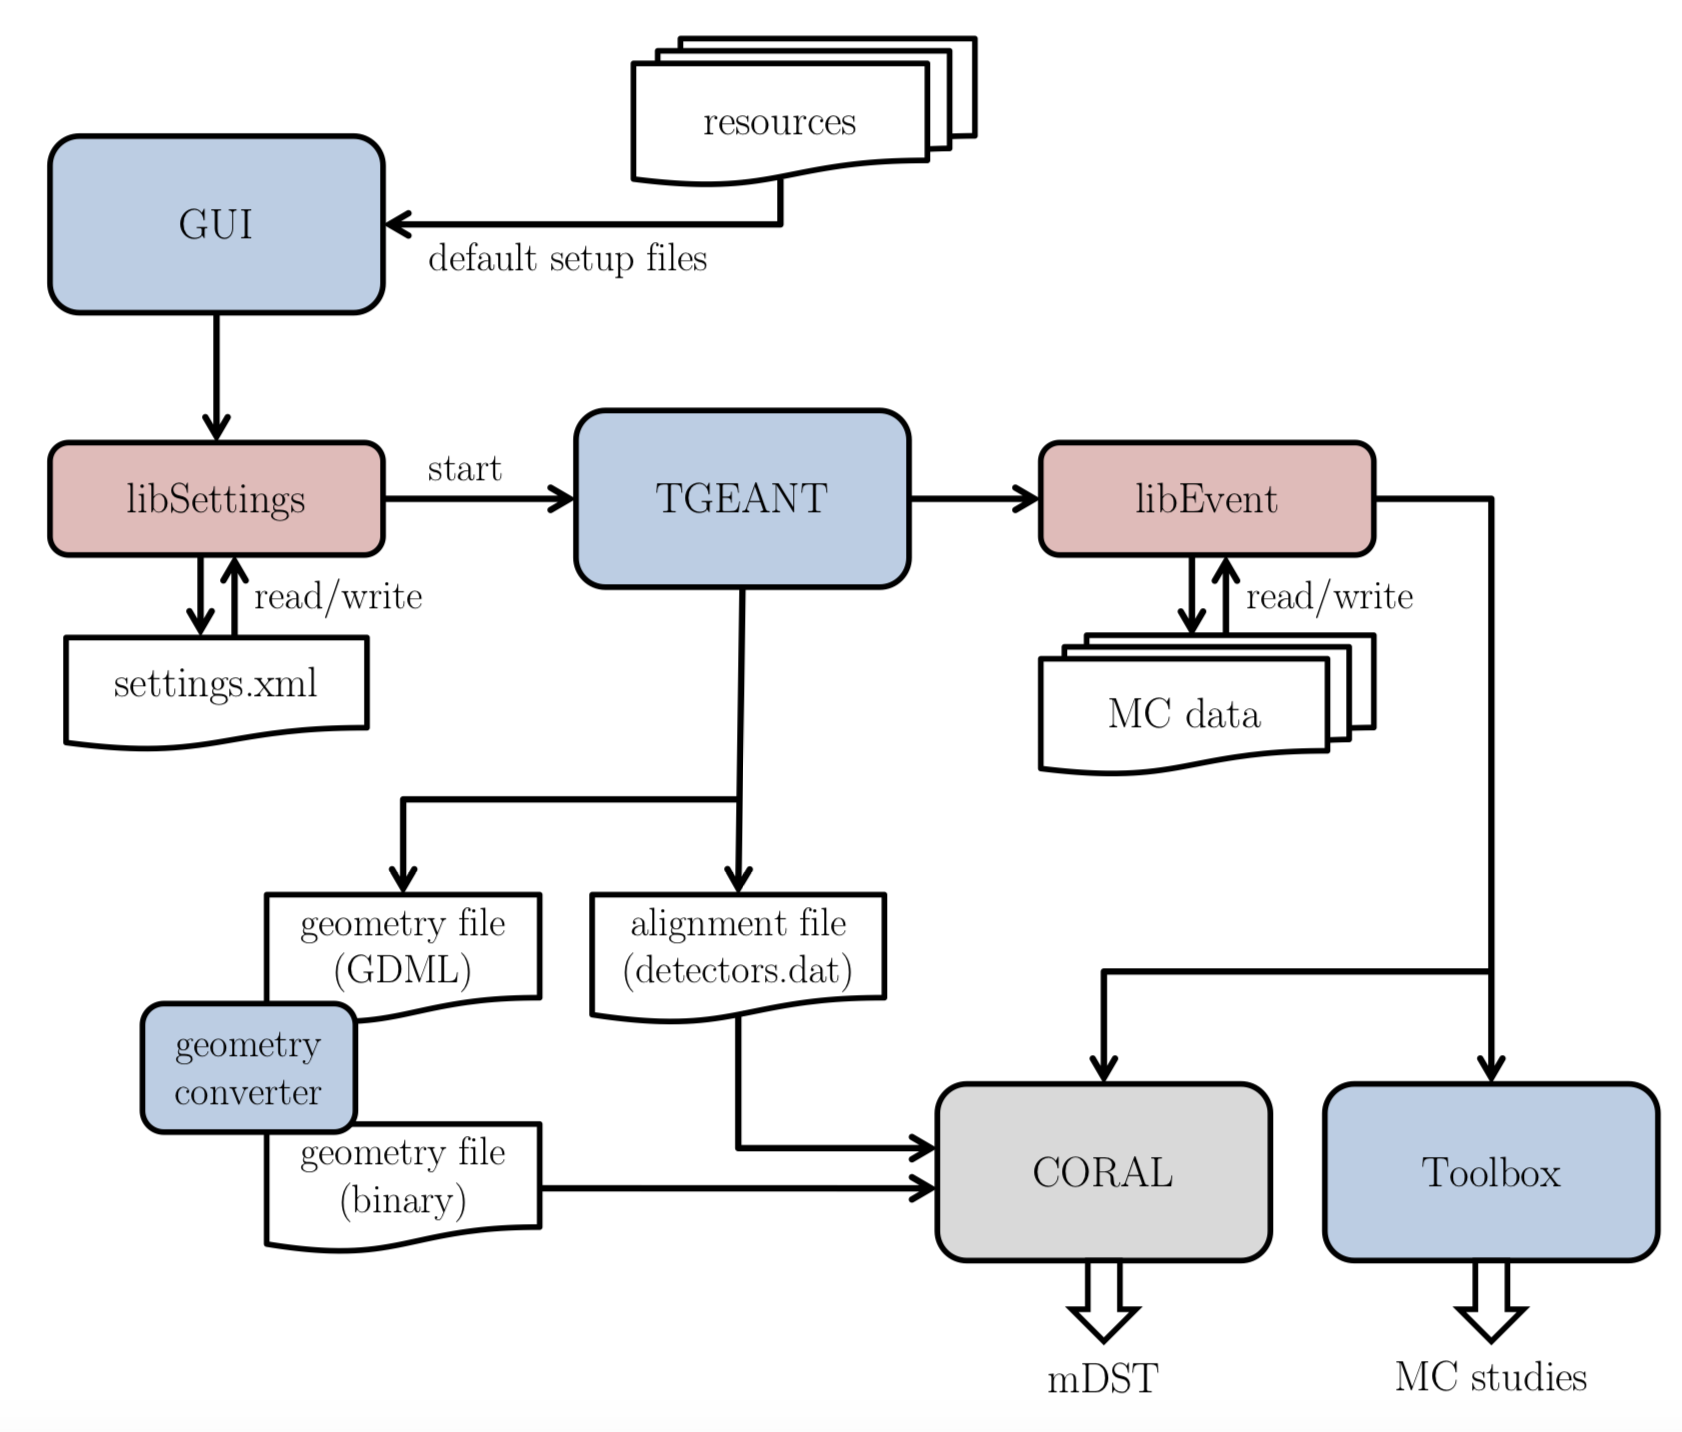
\includegraphics[scale=0.5]{./gfx/TGEANTflowchart.png}
	\caption{Flow chart of the TGEANT software package. The simulation software TGEANT is controlled by a setup file, which is easily created with the graphical user interface. The GUI can draw on different default setup files from the resources folder. The output files can either be analyzed with the Toolbox for the purpose of Monte Carlo studies or processed by CORAL in order to produce mDST files. For the latter case, TGEANT also provides the alignment and geometry files.}
	\label{pic:TGEANTflowchart}
\end{figure}

\subsection{Event simulation}

The event loop in TGEANT is the major part of the simulation software. One or more so-called primary particles are placed with a given momentum vector in the world volume. After the initialization phase, the event loop is started and primary particles are tracked by the Geant4 algorithm through the experimental setup. During the event loop, new particles can only be created by implemented physical processes, applied according to their cross sections. Once the event loop has ended, the output of simulated detector responses is processed. The flow chart of the event loop in TGEANT is illustrated in Fig. \ref{pic:EventLoop}.

\begin{figure}[!h]
  \centering
	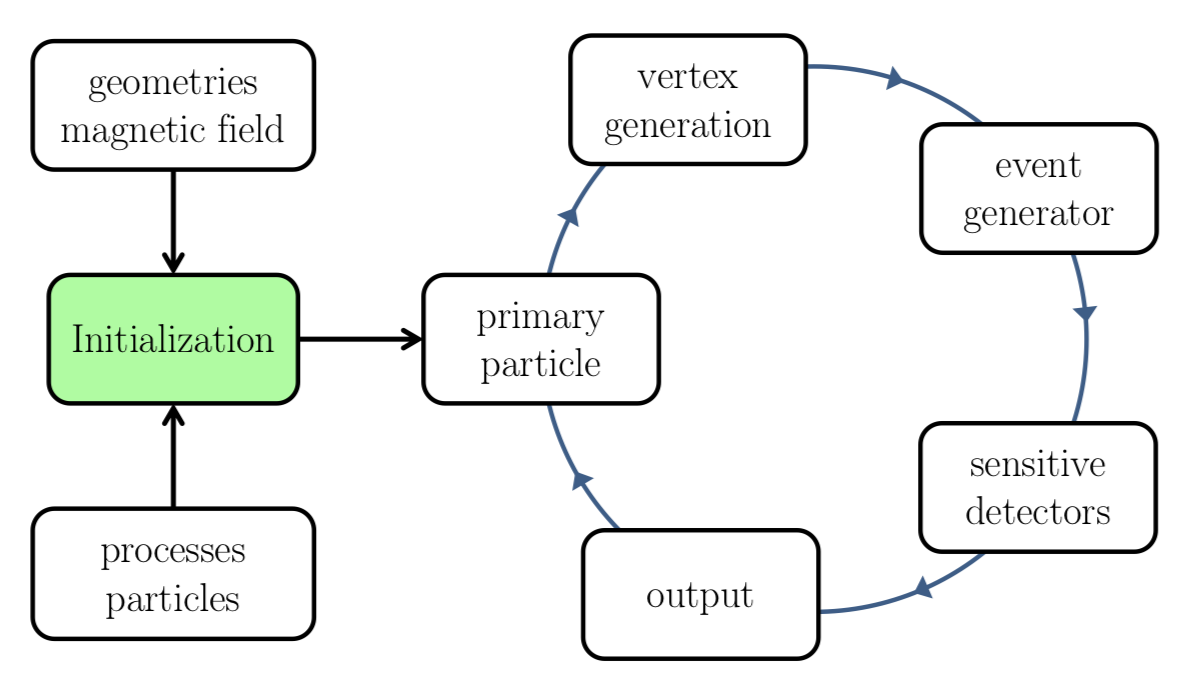
\includegraphics[scale=0.5]{./gfx/EventLoop.png}
	\caption{Flow chart of the event loop in TGEANT.}
	\label{pic:EventLoop}
\end{figure}

\subsection{Primary vertex generation}

The algorithm to generate a primary vertex in TGEANT is responsible for stopping the primary beam particle and for calling an event generator. The \textit{target extrapolation} algorithm is used to trigger the event generator.

The goal of the target extrapolation method is to stop the movement of the primary beam particle at a random position inside the target volume. A flow chart of the method is presented in Fig. \ref{pic:Targetextrap}. It is a multi-purpose method to generate vertices within the target volume. A realistic vertex distribution can easily be simulated by using a beam file and a precise target alignment.
To distinguish between usual detector geometries and target volumes, TGEANT uses the T4TargetBackend system. Each implemented target geometry is derived from this abstract base class. The T4TargetBackend interface is used to gather information about the target that the algorithm needs to work with.

\begin{figure}[!h]
  \centering
	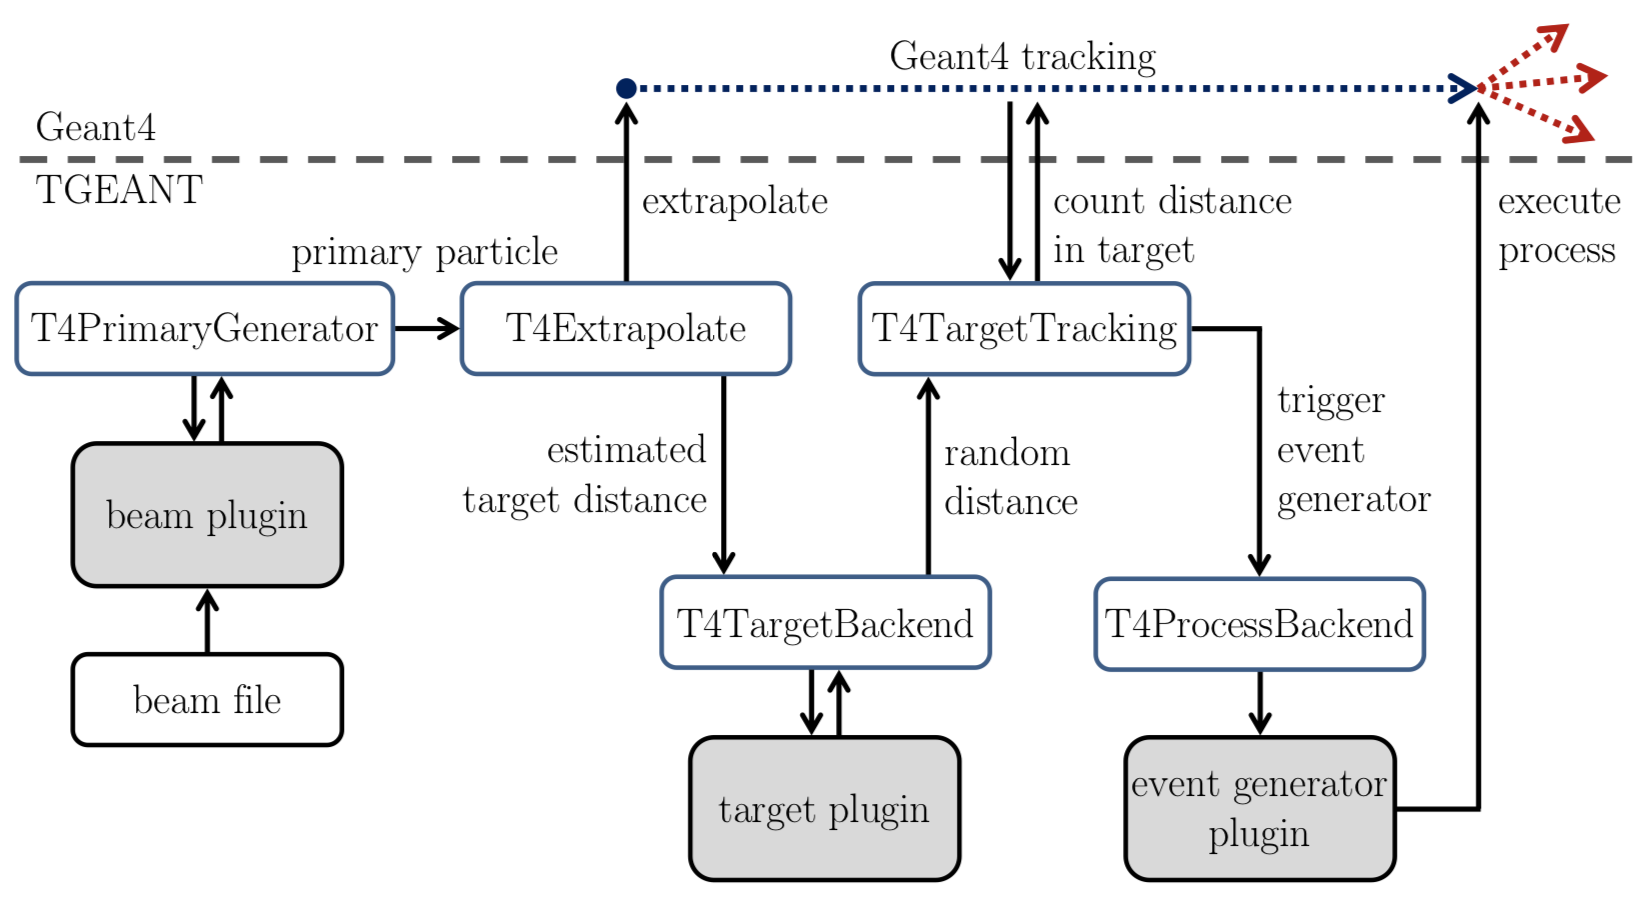
\includegraphics[scale=0.5]{./gfx/Targetextrap.png}
	\caption{Flow chart of the target extrapolation method: The T4Extrapolate class extrapolates the primary particle to the desired starting z position. After traversing a random distance inside the target volumes, the beam particle is stopped by the T4TargetTracking class. At this point, the event generator is applied. This random distance is dictated by the T4TargetBackend derived target class. An estimated distance, which the beam particle is able to traverse in the target volume, is provided by the T4Extrapolate class and can be used optionally.}
	\label{pic:Targetextrap}
\end{figure}

The second key module of the target extrapolation method is the T4TargetTracking class. In the Geant4 tracking algorithm, a particle track is divided into several steps. The T4TargetTracking class allows access to information about the particle’s state, including the particle’s type, the identification number of its track and parent’s track after each step. A unique identification of the primary beam particle is therefore possible. The second part of the information carries the particle’s current momentum, position, and the length of its last step. Even more interesting is the volume where the particle is actually located. Volumes which are marked as active target can be distinguished from all other volumes. The Geant4 tracking algorithm ensures that each particle track creates an intermediate step at each volume boundary. All this together is used to sum up the exact traversed distance of the primary beam particle inside the active target volumes. This allows to trigger the event generator exactly after the beam particle has traversed a random distance inside the target volumes. This method is only feasible if the particle’s maximum step length inside the target volumes is limited. Usually, the step length varies for each step and depends on the particle type and the implemented physical processes and thus also on the surrounding material. Considering a muon in liquid hydrogen, Geant4 chooses a step length in the order of meters and the muon tracking will most likely only be interrupted by the surface crossing. The maximum step length can be tuned in the TGEANT setup file and should be adjusted to the used target volume. For the 2.5 m-long liquid hydrogen target, a maximum step length of 1 mm is used. A shorter distance would not improve the accuracy of the vertex distribution but increase the number of steps and hence suffer in performance.

\subsection{Event generators}

Several interfaces for different event generators are already installed in TGEANT and ready to use, see Fig. \ref{pic:Processbackend}. The event generators are implemented as discrete Geant4 processes using the abstract T4ProcessBackend base class, which handles the interface to TGEANT. This involves the call of the event generator function and the forwarding of the four-momentum of the incoming beam particle at the vertex position.
During particle tracking, all physical processes that a particle is able to do need to propose a step length: the higher the process probability, the shorter the step length. The shortest step length is selected by the Geant4 tracking algorithm for the particle’s next step and the associated process is applied. Consequently, the event generator process, which is implemented in TGEANT as a discrete Geant4 process, also needs to propose a step length during particle tracking. To ensure that this process is never applied by chance, the default proposed step length is 'DBL\_MAX', which is the largest number possible. At the vertex position, however, the proposed step length of the event generator process is changed to zero to ensure that no other process is able to propose a shorter step length and consequently the event generator gets triggered.

\begin{figure}[!h]
  \centering
	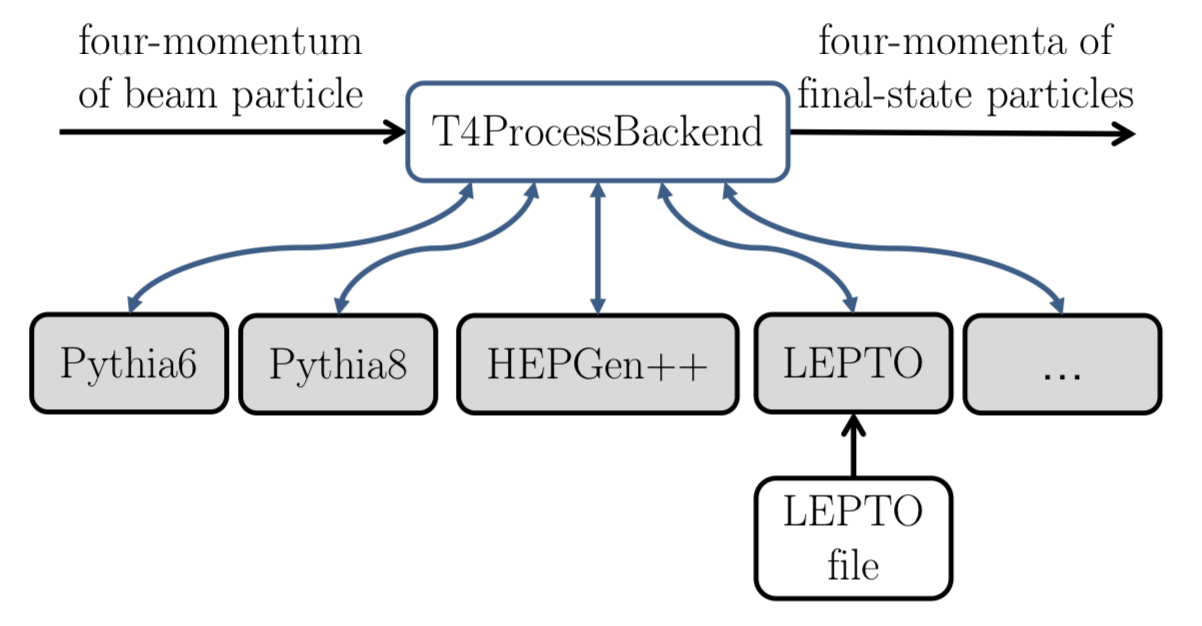
\includegraphics[scale=0.5]{./gfx/Processbackend.png}
	\caption{Inheritance diagram for the T4ProcessBackend base class. The four- momentum of the incoming beam particle is forwarded to the used event generator. The four-momenta of the final state particles are received in return.}
	\label{pic:Processbackend}
\end{figure}

The simplified procedure of an event generator can be described as follows. The four-momentum of the incoming beam particle serves as input parameter and the target nucleon is at rest. During the simulated interaction, one or more outgoing particles are generated. The momentum distribution between these final state particles may be a complex procedure and needs to be randomized by the event generator according to the cross section of the interaction. At the end, however, the energy and momentum conservation needs to be ensured and TGEANT has to exchange the initial state beam particle with all final state particles.


%----------------------------------------------------------------------------------------

\section{DJANGOH as a physics generator for TGEANT}

The original DJANGOH is a FORTRAN framework. The main problem I encountered is that DJANGOH was supposed to be used in the Monte-Carlo simulation of the COMPASS apparatus, TGEANT. As the whole simulation is implemented in C++, the inclusion of a new generator inside the chain is done via the integration of a plugin in C++ containing the generator. Thus, in order to include DJANGOH into TGEANT, I had to modify DJANGOH so that it can be used as a C++ plugin generator by TGEANT.

There are two ways to implement a generator in TGEANT :
\begin{itemize}
\item As an internal generator (Pythia and HEPGEN++ way) : a C++ interface to the
generator is needed, the conservation of $P(p,E)$ is perfect and it only needs a
beamfile for the primary generator.
\item As an external generator (Lepto) : the beamfile is read by the standalone
generator, the primary generation and process infos are stored inside a file and
TGEANT has to do an extrapolation to -9 meters as the primary generation was done
outside of it, occasioning $P(p,E)$ being not perfectly conserved.
\end{itemize}

The external implementation is quite complicated as three classes are needed in order
to use the generator in TGEANT. First, the beamfile has to be read by the generator
which then outputs a file containing the beamfile infos but in its own format.
Then a first class has to be dedicated to the reading of the beamfile, recovering
the information about the selected muon in the file. A second class takes care of
passing of information between the generator and TGEANT. The last class is the
class of the generator itself (Fig. \ref{fig:leptoex}).

\begin{figure}[!htb]
\centerline{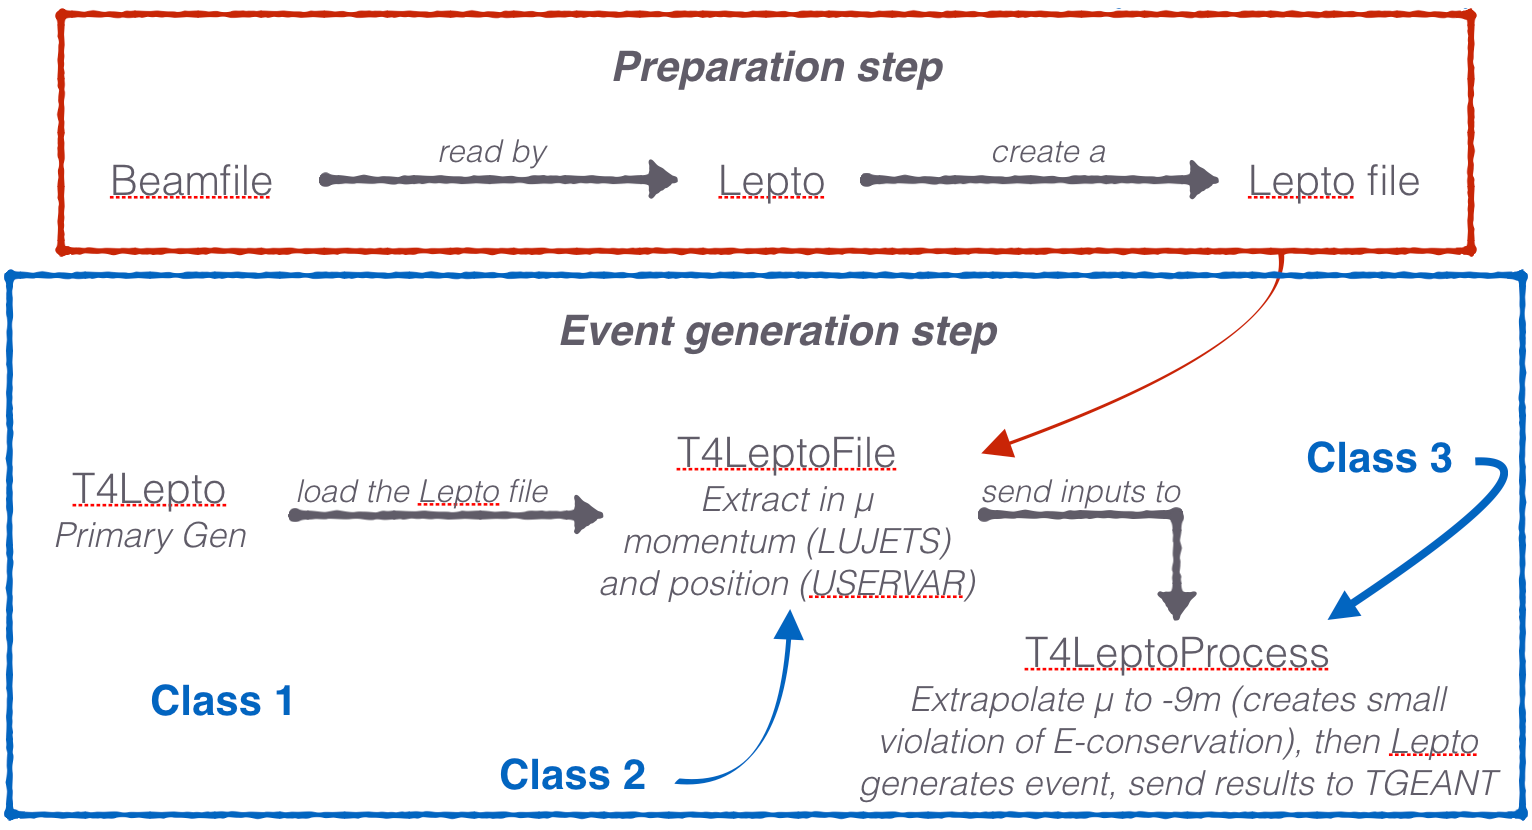
\epsfig{file=gfx/leptoex.png,width=12cm}}
\caption{Diagram explaining the philosophy of the external generator implementation, taking the
implementation of LEPTO as an example. First and foremost, a specific beamfile is created after the
initial one. The external generator will read this pregenerated file to extract infos about the incoming
particle. As these informations are at the interaction point, a backward propagation extrapolation in the
target material has to be made, inducing some small violations of energy conservation.
Then the generator is producing the event and sends the results to TGEANT.}\label{fig:leptoex}
\end{figure}

If you apply this method to DJANGOH, then you encounter several critical problems :
\begin{itemize}
\item A new file format for the converted beamfile has to be created.
\item DJANGOH has to be modified to allow backward propagation of the incoming muon.
\item The result of fragmentation (LUJETS) has to be recovered in a file.
\end{itemize}
This results in many file accesses and consequently it is a non-efficient way to
implement DJANGOH inside TGEANT.

The internal implementation recquires perhaps more work on the generator itself however
this solution is much more efficient. Here, only two class are needed. One is the
interface class that creates instances of DJANGOH that can be manipulated in any C++
environment. This class is a C++ interface that is handling the FORTRAN part of DJANGOH.
The other class is taking care of passing the information between the interface to the
generator and TGEANT (Fig. \ref{fig:pythiaex}).

\begin{figure}[!htb]
\centerline{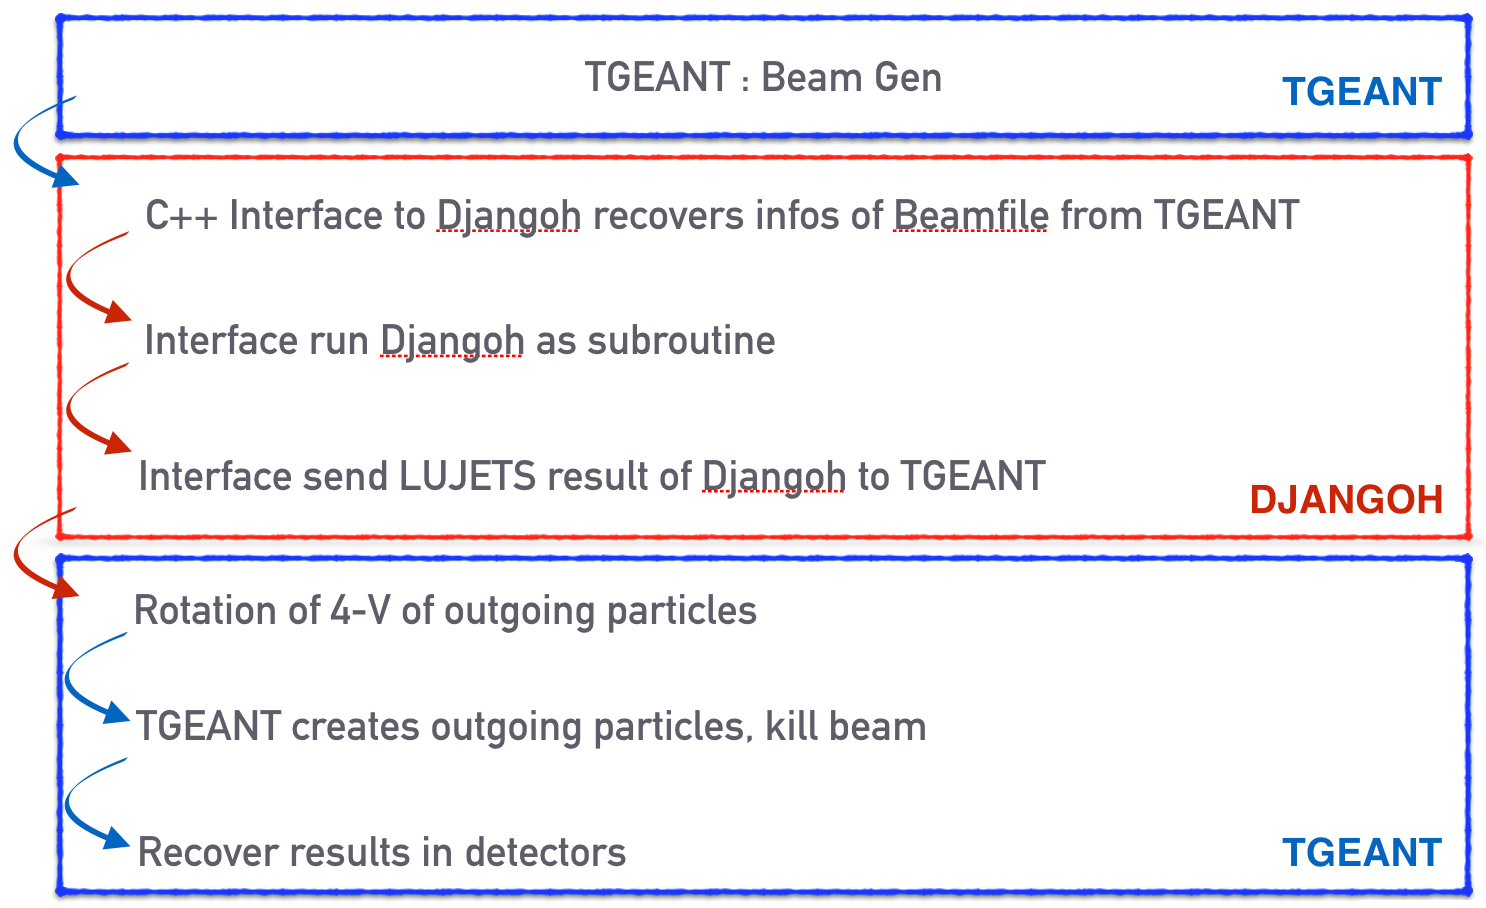
\epsfig{file=gfx/pythiaex.png,width=12cm}}
\caption{Diagram explaining the philosophy of the internal generator implementation.
The beamfile is read by TGEANT and the C++ interface to the generator is recovering the
informations of the incoming particle. This interface then runs the generator as a subroutine
and sends back the results of the generation to TGEANT, which then creates the outgoing particles
accordingly.}\label{fig:pythiaex}
\end{figure}

This second method was used to implement DJANGOH inside TGEANT.

%----------------------------------------------------------------------------------------

\section{Results on electroproduction from photon conversion}

At this point, with DJANGOH fully integrated as an event generator for TGEANT, we can go back to our original goal : see if DJANGOH describes better the electroproduction from photon conversion at COMPASS than RADGEN did. Looking again at the absolute value of the $\Phi$ angle in the $\gamma$-nucleon reference frame, we see an improvement compared to the factor 1.8 difference seen with RADGEN. The discrepancy is only of the order of 10\% at $|\Phi| \sim 0$ and less than 5\% elsewhere; showing that DJANGOH is able to reproduce with a good fidelity the electroproduction from photon conversion observed in data.

\begin{figure}[!h]
  \centering
	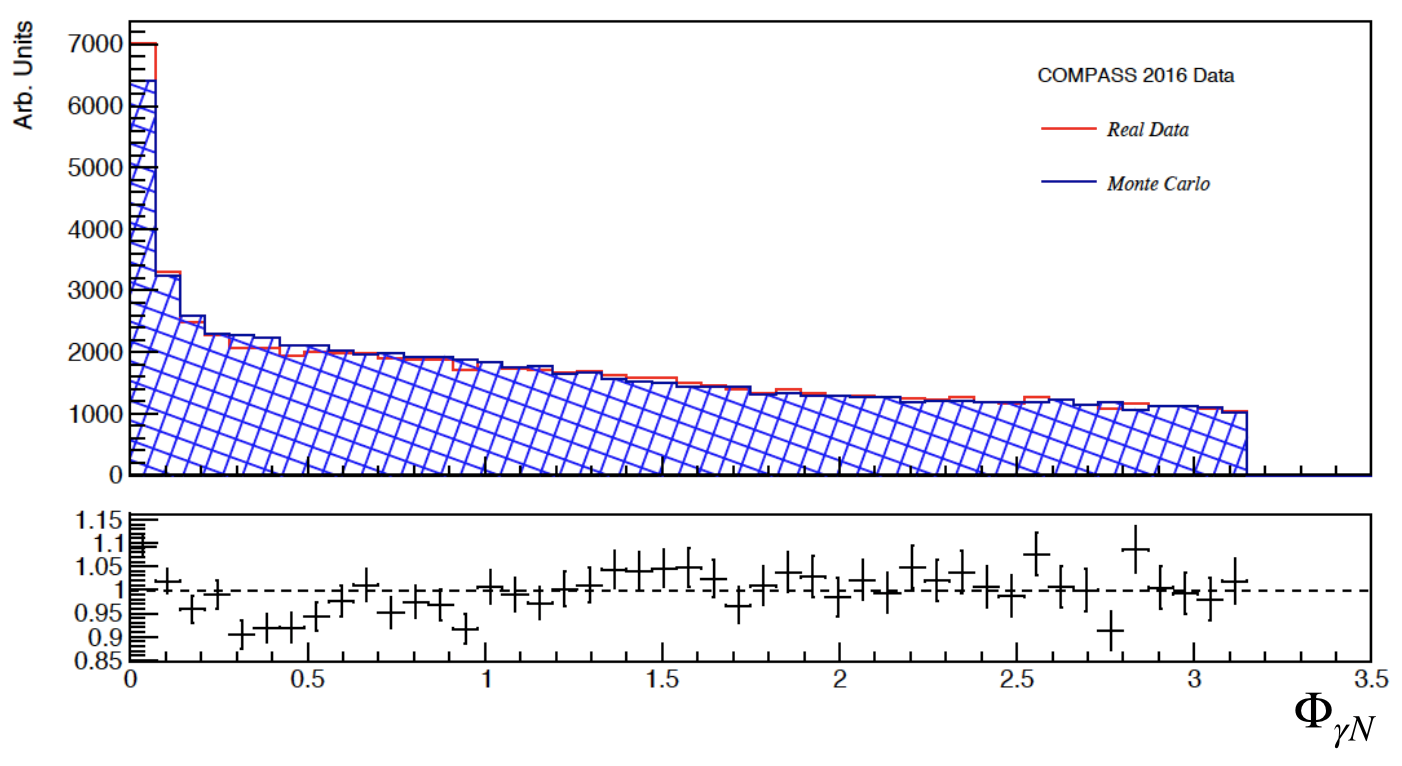
\includegraphics[scale=0.6]{./gfx/Eprod2016.png}
	\caption{Electron distribution versus $\Phi$ in the $\gamma$-nucleon reference plane for 3 $< p_e <$ 8 GeV (region where RICH can discriminate electron in real data). Real Data are in red, Monte-Carlo with DJANGOH in blue, with the ratio data over MC on the bottom panel.}
	\label{pic:Eprod2016}
\end{figure}

%----------------------------------------------------------------------------------------

\section{Summary}

TGEANT is a flexible Monte Carlo simulation which allows a precise reproduction of the experimental setup. This flexibility allows one to use the event generator one sees fit to his needs, choosing between the internal or external implementation of this generator to the simulation. DJANGOH, after being integrated as an internal generator inside TGEANT, shows good performances in the data versus MC comparison, especially when comparing the electroproduction from photon conversion, being more accurate than previously used generator RADGEN.
